%%
% summary landscape plots
%
      \begin{figure*}[t]
        \centering
        \begin{subfigure}[b]{0.45\textwidth}
            \centering
            \caption[]%
            {{\small Netpipe 64 KB message}}  
            \vspace*{-0.3cm}
            %\hspace*{0.35cm}  
            \label{fig:netpipe64Kov}
            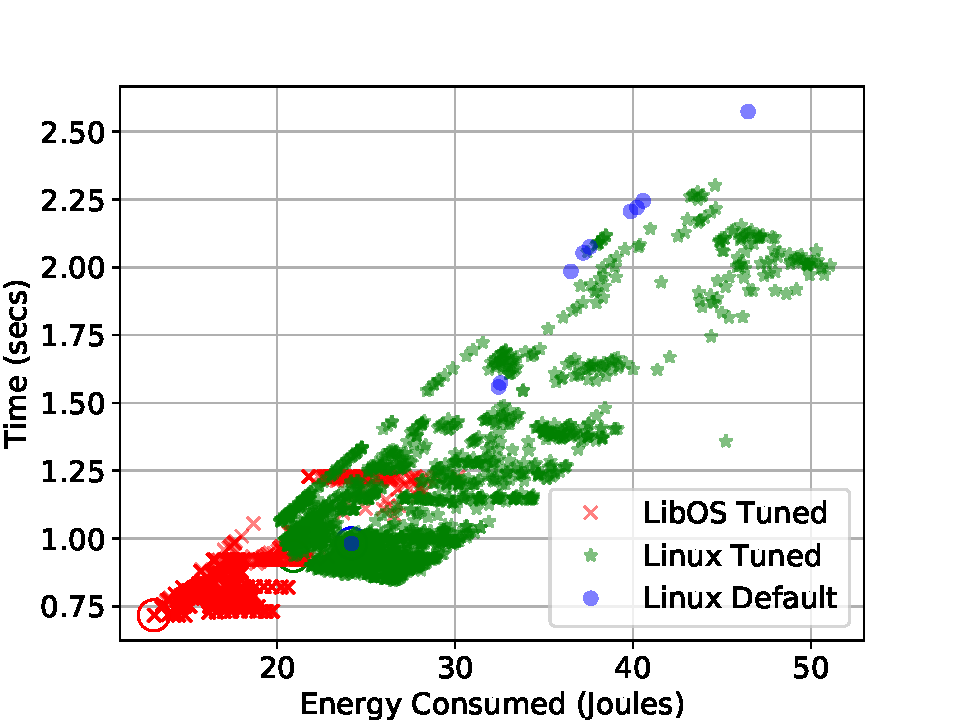
\includegraphics[width=\textwidth]{osdi_figures/netpipe_65536_overview.pdf}
        \end{subfigure}
%        \hfill
        \begin{subfigure}[b]{0.45\textwidth}  
            \centering 
            \caption[]%
            {{\small Memcached 600K QPS}} 
            \vspace*{-0.25cm}    
            \label{fig:mcdov}
            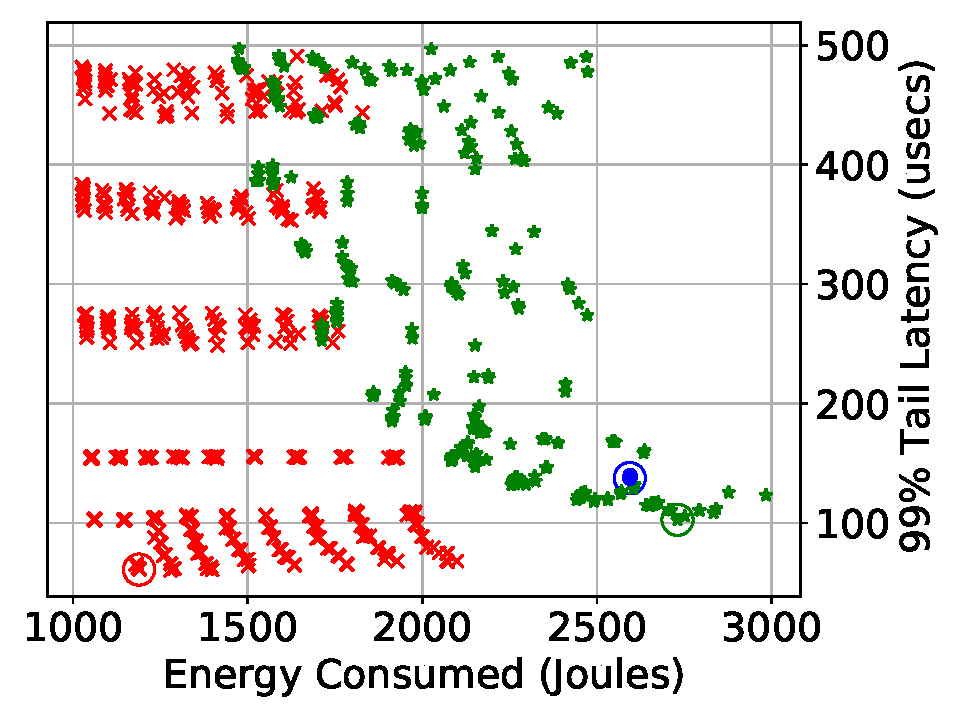
\includegraphics[width=\textwidth]{osdi_figures/mcd_600000_overview.pdf}
        \end{subfigure}
        \vskip\baselineskip
        \vspace*{-0.47cm} 
        \begin{subfigure}[b]{0.45\textwidth}   
            \centering 
            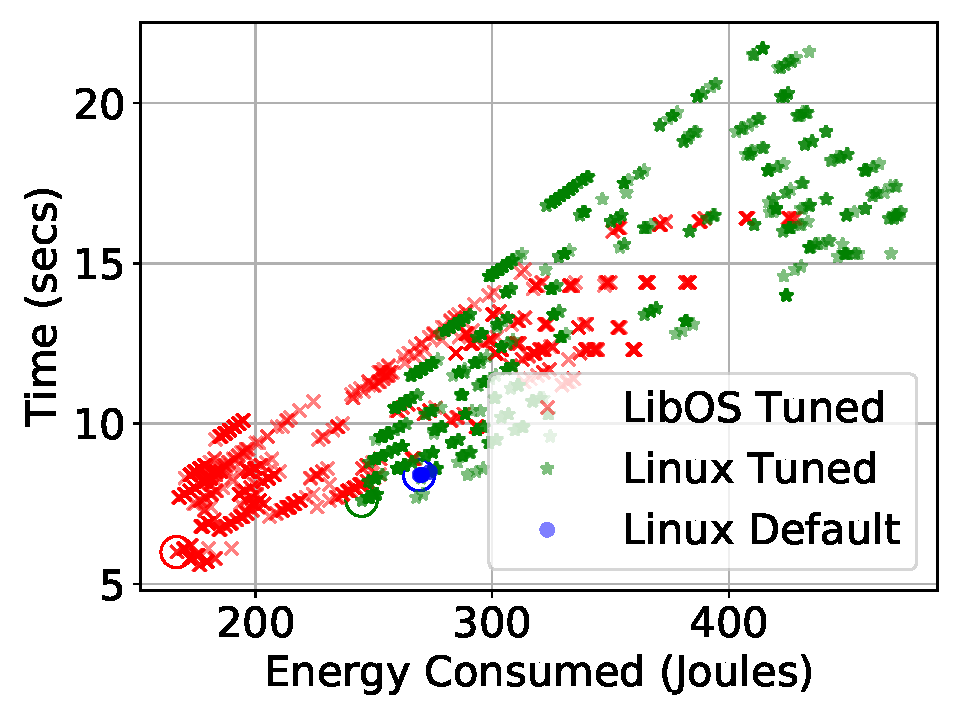
\includegraphics[width=\textwidth]{osdi_figures/nodejs_overview.pdf}
            \caption[]%
                    {{\small NodeJS 100K requests}}
                    %\hspace*{0.35cm}  
            \label{fig:nodejsov}
        \end{subfigure}
%        \hfill
        \begin{subfigure}[b]{0.45\textwidth}   
            \centering 
            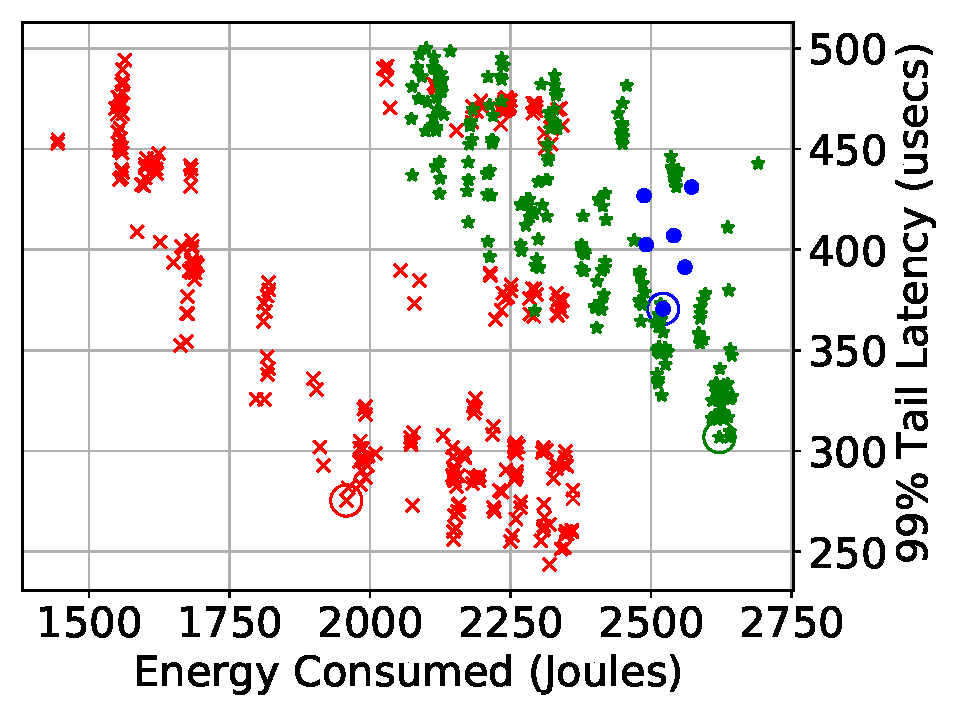
\includegraphics[width=\textwidth]{osdi_figures/mcdsilo_200000_overview.pdf}
            \caption[]%
            {{\small Memcached-silo 200K QPS}}    
            \label{fig:mcdsiloov}
        \end{subfigure}
        \caption[]
                {\small
These landscape plots portray the space of energy-performance profiles
that an OS/workload software stack can exhibit. The circle around individual points represent the min EPP values achieved in each workload.
\textit{Note that, in these plots, the origins do not start at zero
because the aim of the plots is to highlight structure within a plot
rather than to draw a comparison across plots.}
                  %Data from a run the settings associated with the 'best' EPP points are presented in~\ref{sec:data} and discussed in~\ref{sec:details}.          %Using these values we plot a timeline of the joule readings for one experimental run at the setting for Linux tuned and libOS along with data from a default Linux run of the workload.  The x-axis is the time offset from the beginning of the experiment.  For each log entry with a joule reading, we plot its value against its timestamp offset from the beginning of the run.  While the log has entries for every interrupt, we restrict sampling the joule counter to be at least 1ms apart as per the hardware manual's recommendation, as such not all log entries have an associated joule value.  To improve readability we only show a subset of the markers and use a line to connect the visible marks to the points not shown.    
        } 
        \label{fig:overview}
    \end{figure*}



Figure~\ref{fig:overview} illustrates energy-performance landscapes that summarize all the experiments for four of the eleven workloads runs (~\ref{table:wrkcfgs}).  Each point in these graphs represents a single experimental run.  Using log data for a run, we calculate the total energy consumed along with a workload-specific performance measure. For both memcached and memcached-silo, we filter any results that do not satisfy an SLA of 500 $\micro s$. In the performance metrics of both closed loop and open loop workloads, better in both cases is indicated by a lower value. Therefore, the best performance and energy states form a pareto-optimal energy-performance curve of points that are closest to the origin in the landscape plots.  

%In netpipe and nodejs, the workload-specific measure we use is the time taken to complete a fixed number of sequential transactions in a closed-loop setting.  For netpipe (figure~\ref{fig:netpipe64Kov}), we measure the time taken to complete 5000 round-trips between a client and server configured with the same OS and hardware settings for a fixed message size of 64 KB.  For nodejs (figure ~\ref{fig:nodejsov}), we measure the time required to serve 100,000 HTTP requests.

%In the open-loop workloads, memcached and memcached-silo, the performance metric used is the 99\% tail latency specific queries-per-second (QPS) load sustained for a period of 20 seconds.
%In memcached (figure~\ref{fig:mcdov}), we apply an offered load of 600K QPS generated using the ETC Facebook benchmark~\cite{mutilate}.
%For memcached-silo (figure~\ref{fig:mcdsiloov}), we apply a load of 200K QPS. Note that, in both open-loop cases, the offered loads are close-to but do not exceed the maximum system's capacity (~\ref{sec:perf_baseline}).  
%Furthermore, for both memcached and memcached-silo, we filter any results that do not satisfy an SLA of 500 $\micro s$.  
%Each experimental run uses a unique setting for the three hardware settings we study (ITR, DVFS, and RAPL).

%Given that we use total time for a fixed amount of work in the close loop settings and we use 99\% tail latency in the open loop settings as performance metrics, better in all cases is indicated by a lower value. The relative value of one point versus another in figure~\ref{fig:overview} depends on what value/utility one places on the importance/cost of energy versus performance.


To enable analysis we will use the product of Energy and Performance  (EPP), as a single quantity ($Joules \times Performance$) to rank points. EPP is one simple way of comparing individual results as points with lower EPP represent a systems ability to achieve an overall better result in the tradeoff space. Figure~\ref{fig:overview} also include circles drawn around the points with the overall min EPP achieved for the each OS configuration studied. Across all the workloads, tuning libOS was able to achieve up to 74\% EPP savings over Linux. In section~\ref{sec:q1_2} we will examine how differences in OS path length and efficiency plays a role in these results. We also find that tuning Linux could achieve EPP savings up to 48\% over its default behavior. This demonstrates, independent of OS design and implementation changes a general purpose OS can do better on a dedicated workload with a simpler static policy.

%The landscape plots suggests that the OS has a fundamental influence on the energy-performance profile that can be achieved over the range of the three hardware settings swept.  Running a dedicated application with a libOS structure results in significant pareto-optimal energy-performance benefits. In all the landscapes plots, including those not shown, the library OS has a pareto-optimal curve that is closet than that of the Linux.  The gap is unsurprinsgly less pronounced for the open loop workloads at the lowest load. 

The landscape plots also reveal that the OS response to the various settings has two interesting phenomena.  First, both OS' have a relatively clear pareto-optimal curve that identifies the setting for which there exists energy performance tradeoffs that an administrator might want to exploit. A system with only one point at a lower EPP may not be as useful as a system that has many distinct points at similar EPPs; such points allow tuning for one's utility and cost or adjust to changes in utility and costs. Second, we can see more distinct structure within the libOS in the open loop workloads~\ref{fig:mcdov}~\ref{fig:mcdsiloov}, we find these small bands are placed by their respective ITR-delay values and the small points within each band is a search through DVFS and RAPL space. We attribute the simplicity of the libOS to demonstrating this structure, which argues policies built in the libOS can be simpler and more effective.
%Second, someone hoping to tune manually or in an automated fashion should be aware that many settings do not fall on the parateo-optimal curve and care must be taken to avoid choosing bad settings.
 
%functionality of the OS plays by examining the more detailed data.  

%When only considering EPP we found across the sweep of the three hardware parameters across all the workloads the best EPP achieved by the library OS was from X to Y better than the best EPP achieved with Linux.  

%Focusing on the Tuned Linux points in comparison to the default Linux behaviour



%Linux's default behaviour is closest to the optimal behaviour achieved with a static tuning in Memcached.  On the other workloads as visible in the landscapes the default behaviour can suffer high variability, which swings its realized energy or time quite far from optimal, or even if stable its mean can still be suboptimal.  To see this consider figure~\ref{fig:mcdov}.  While the default points are tightly clustered if the same tail latency could be achieved via manual tuning for approximately 400 less Joules over the 20 second period (using the horizontal intercept of the default cluster at P,Q the furthest left Tuned Linux point M,N represents equivalent tail latency at an energy consumption of M).

%More generally comparing best case mean EPPs we observed, across all workloads that statically tuning Linux results in X-Y\% lower EPP compared to how its default behaviour.  

% to do not sure this belongs here on in the discussion. 
%The above observation suggests that the complex OS energy management, design and implementation, do not easily result in optimal behaviour for a fixed workload.  While static tuning can improve the behaviour it is hard to tell how much better the results could be if dynamic energy management were more systemically removed or turned off.  In some sense the library OS does represent such a contrast but it of course is a more radical departure.  

  
 %todo it would be nice to quantify EPP ranges and how many diverse settings have equivalent EPPs as this is also very cool to know... can't be told from the landscapes as we can't see the settings... this is really a more detailed finding but global in a data sense. 

%Discuss any other overview details here that don't easily fit in the analysis section.



